\documentclass[a4paper,12pt]{article}
\usepackage{amssymb} % needed for math
\usepackage{amsmath} % needed for math
\usepackage[utf8]{inputenc} % this is needed for german umlauts
\usepackage[english]{babel} % this is needed for german umlauts
\usepackage[T1]{fontenc}    % this is needed for correct output of umlauts in pdf
\usepackage[margin=2.5cm]{geometry} %layout
\usepackage{listings} % needed for the inclusion of source code
\usepackage{subcaption}

% the following is needed for syntax highlighting
\usepackage{color}

\definecolor{dkgreen}{rgb}{0,0.6,0}
\definecolor{gray}{rgb}{0.5,0.5,0.5}
\definecolor{mauve}{rgb}{0.58,0,0.82}

\lstset{ %
  language=Java,                  % the language of the code
  basicstyle=\footnotesize,       % the size of the fonts that are used for the code
  numbers=left,                   % where to put the line-numbers
  numberstyle=\tiny\color{gray},  % the style that is used for the line-numbers
  stepnumber=1,                   % the step between two line-numbers. If it's 1, each line
                                  % will be numbered
  numbersep=5pt,                  % how far the line-numbers are from the code
  backgroundcolor=\color{white},  % choose the background color. You must add \usepackage{color}
  showspaces=false,               % show spaces adding particular underscores
  showstringspaces=false,         % underline spaces within strings
  showtabs=false,                 % show tabs within strings adding particular underscores
  frame=single,                   % adds a frame around the code
  rulecolor=\color{black},        % if not set, the frame-color may be changed on line-breaks within not-black text (e.g. commens (green here))
  tabsize=4,                      % sets default tabsize to 2 spaces
  captionpos=b,                   % sets the caption-position to bottom
  breaklines=true,                % sets automatic line breaking
  breakatwhitespace=false,        % sets if automatic breaks should only happen at whitespace
  title=\lstname,                 % show the filename of files included with \lstinputlisting;
                                  % also try caption instead of title
  keywordstyle=\color{blue},          % keyword style
  commentstyle=\color{dkgreen},       % comment style
  stringstyle=\color{mauve},         % string literal style
  escapeinside={\%*}{*)},            % if you want to add a comment within your code
  morekeywords={*,...}               % if you want to add more keywords to the set
}

% this is needed for forms and links within the text
\usepackage{hyperref}
\usepackage[toc,page]{appendix}

\usepackage{tikz}
\usepackage{pgfplots}

%%%%%%%%%%%%%%%%%%%%%%%%%%%%%%%%%%%%%%%%%%%%%%%%%%%%%%%%%%%%%%%%%%%%%%
% Variablen                                                          %
%%%%%%%%%%%%%%%%%%%%%%%%%%%%%%%%%%%%%%%%%%%%%%%%%%%%%%%%%%%%%%%%%%%%%%
\newcommand{\authorName}{Ali Asgari Khoshouyeh (Student \#24868739)}
\newcommand{\tags}{\authorName, my, tags}
\title{CPEN 502 Assignment-b: Reinforcement Learning (Look Up Table)}
\author{\authorName}
\date{\today}

%%%%%%%%%%%%%%%%%%%%%%%%%%%%%%%%%%%%%%%%%%%%%%%%%%%%%%%%%%%%%%%%%%%%%%
% PDF Meta information                                               %
%%%%%%%%%%%%%%%%%%%%%%%%%%%%%%%%%%%%%%%%%%%%%%%%%%%%%%%%%%%%%%%%%%%%%%
\hypersetup{
  pdfauthor   = {\authorName},
  pdfkeywords = {\tags},
  pdftitle    = {Reinforcement Learning (Look Up Table)}
}

%%%%%%%%%%%%%%%%%%%%%%%%%%%%%%%%%%%%%%%%%%%%%%%%%%%%%%%%%%%%%%%%%%%%%%
% THE DOCUMENT BEGINS                                                %
%%%%%%%%%%%%%%%%%%%%%%%%%%%%%%%%%%%%%%%%%%%%%%%%%%%%%%%%%%%%%%%%%%%%%%
\begin{document}

\maketitle

\section*{Team Members}
We are a team of three sharing the same code base. 
\begin{itemize}
\item Christina Sun
\item Husna Kalim
\item Ali Asgari Khoushouyeh
\end{itemize}


It is noteworthy to mention that close to the extended deadline we realized that our code is orders of magnitude slower on my teammates' machines. So we sharing the plot data too. 
\pagebreak
\section*{(4) The use of a neural network to replace the look-up table and approximate the Q-function has some disadvantages and advantages.}
\subsection*{a) There are 3 options for the architecture of your neural network. Describe and draw all three options and state which you selected and why. (3pts)}

\begin{figure}[ht]
  \subfloat[Action as output\label{fig:first_architecture}]{
   \begin{minipage}[c][1\width]{
      0.3\textwidth}
     \centering
      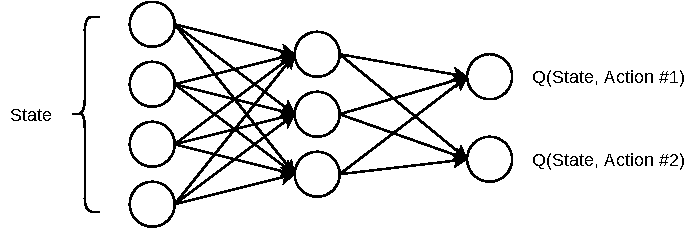
\includegraphics[width=1\textwidth]{drawio/1.pdf}
  \end{minipage}}
 \hfill  
  \subfloat[Action as input\label{fig:second_architecture}]{
   \begin{minipage}[c][1\width]{
      0.3\textwidth}
      \centering
      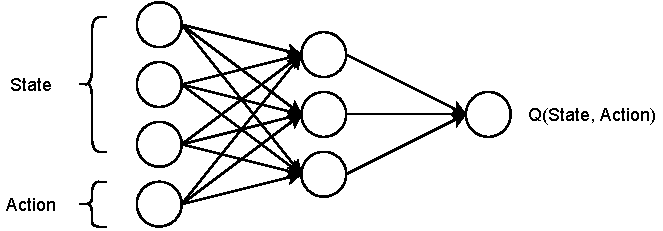
\includegraphics[width=1\textwidth]{drawio/2.pdf}
   \end{minipage}}
 \hfill  
  \subfloat[Adding time dimention\label{fig:third_architecture}]{
   \begin{minipage}[c][1\width]{
      0.3\textwidth}
      \centering
      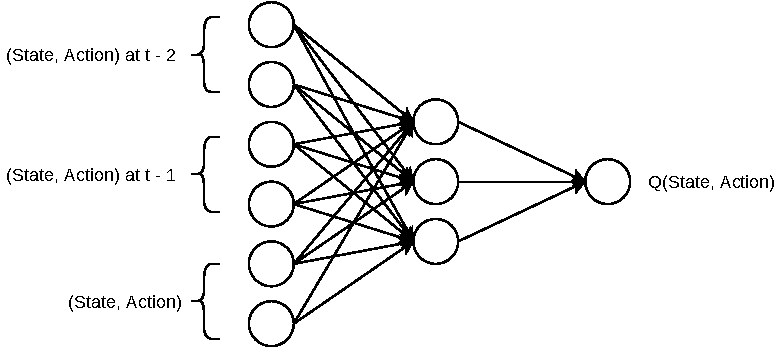
\includegraphics[width=1\textwidth]{drawio/3.pdf}
   \end{minipage}}
\caption{Different architectures considered for the neural network as the function approximator for the Q values of different game actions.}
\label{fig:architectures}
\end{figure}
FIg. \ref{fig:architectures} shows the different architectures we considered for our neural network to be plugged in instead of the lookup table. The first two architectures shown in Fig. \ref{fig:first_architecture} and Fig. \ref{fig:second_architecture} are the ones discussed in the class. The first one codes the Q value for different possible actions at each step as different neurons of the output. In the second architecture the action is coded as some input neurons and the Q value corresponding the the encoded action as the input at a certain state is coded as the single output neuron. 

The novel architecture that we used is the one shown in Fig. \ref{fig:third_architecture} which is essentially same as the second architecture, but, it also receives the state-actions of the two past time-steps as input. This is following our intuition used in the second part of the assignment where we included the past two state-actions in the lookup table keys to capture the delay of rewards as it may take some time for a bullet to hit the enemy and get reflected in the reward policy. 

\pagebreak
\subsection{b) Show (as a graph) the results of training your neural network using the contents of the LUT from Part 2. Your answer should describe how you found the hyper-parameters which worked best for you (i.e. momentum, learning rate, number of hidden neurons). Provide graphs to backup your selection process. Compute the RMS error for your best results. (5 pts)}

\begin{table}[hbt!]
\centering
\begin{tabular}{c|c|c|c}
Learning Rate &  Momentum &  Hidden Neurons & RMSE\\
\hline
1.00E-04 &0 & 5 & 9.666091389\\
1.00E-04& 0 &  15 &  9.660078042\\
1.00E-04 &  0 &  30 & 9.628909289\\
0.001 &  0 &  5 &  7.632740399\\
0.001 &  0 &  15 &  6.943443362\\
0.001 &  0 &  30 &  6.711401519\\
0.01 &  0 &  5 &  7.985192317\\
0.01 &  0 &  15 &  7.018144655\\
0.01 &  0 &  30 &  6.530952131\\
1.00E-04 &  0.5 &  5 &  9.148578254\\
1.00E-04 &  0.5 &  15 &  8.993952348\\
1.00E-04 &  0.5 &  30 &  9.051175005\\
0.001 &  0.5 &  5 & 7.297405961\\
0.001 &  0.5 &  15 &  \textbf{6.335407802}\\
0.001 &  0.5 &  30 &  \textbf{6.289893926}\\
0.01 &  0.5 &  5 &  7.919711744\\
0.01 &  0.5 &  15 & 7.75168296\\
0.01 &  0.5 &  30 &  8.222388904\\
1.00E-04 &  0.9 &  5 &  7.713839065\\
1.00E-04 &  0.9 &  15 & 6.790881731\\
1.00E-04 &  0.9 &  30 & 6.754064308\\
0.001 &  0.9 &  5 &  7.772037228\\
0.001 &  0.9 &  15 &  7.099569645\\
0.001 &  0.9 &  30 &  6.728784713\\
0.01 &  0.9 &  5 &    11.50926595\\
0.01 &  0.9 &  15 &  13.85358874\\
0.01 &  0.9 &  30 &  18.89859967\\

\end{tabular}
\caption{RMSE after 100 epochs under different hyperparameter values for training the neural network on the static lookuptable data.}
\label{tbl:grid_search}
\end{table}

We performed a grid search on different possible values of number of hidden neurans, momentum and learning reate. The results are shown in Table \ref{tbl:grid_search}. As the difference between 15 hidden neurons and 30 hidden neurons (shown bolded in the table) is negligible, we keep 15 nerons as it is much faster. 

\begin{figure}[hbt!]
\begin{tikzpicture}
    \begin{axis}[
        xlabel=epochs,
	 height = 10cm,
        width=\textwidth,
        ylabel=RMSE,
	 ymin=0,
        xticklabel style={rotate=30},       
	 xlabel style={yshift = -20pt}
]
    \addplot[smooth,mark=.,blue] table {static_lut.dat};
    \addlegendentry{Momentum = 0.5, Learning Rate = 0.5, Hidden Neurons  = 15}
    \end{axis}
    \end{tikzpicture}
\caption{The convergence of the select hyperparameters over static lookup table data.}
\label{fig:static_lut}
\end{figure}

We show the convergance of the selected settings in Fig. \ref{fig:static_lut}. It shows that our neural network is able to reduce the error fitting on the lookup table static data by decreasing the error from more than 6 to around \textbf{4}. 

\pagebreak

\subsection*{c) Comment on why theoretically a neural network (or any other approach to Q-function approximation) would not necessarily need the same level of state space reduction as a look up table. (2 pts)}
As an example, we are using the distance to the enemy as one of the dimensions of the states. When using a lookup table, it matters to decrease the number of possible values to few, so the number of entries in the lookup table do not blow up and the get revisited often. But as the neural network treats the input as a real number and does not do exact-match like the lookup table, close values also let the states be somehow recalled by the neural network. Thus, using the large number of possible values for the distant to enemy is still tractable by the neural network. That said, it is still important to limit the range of that value to something close to the other inputs so the weight initialization would fit this dimension like the other dimensions. 

\pagebreak
\section*{(5) Hopefully you were able to train your robot to find at least one movement pattern that results in defeat of your chosen enemy tank, most of the time.}

\subsection*{Identify two metrics and use them to measure the performance of your robot with online training. I.e. during battle. Describe how the results were obtained, particularly with regard to exploration? Your answer should provide graphs to support your results. (5 pts)}

We measure the following metrics:

\begin{enumerate}
\item \textbf{Win rate}: the number of rounds won among 100 rounds. 
\item \textbf{Win turns}: the average number of turns it takes our robot to defeat the enemy. We calculate this average only for the won rounds. Lower values are better as it means our robot is able to kill its opponent more quickly. 

\end{enumerate}

We interleave battles of training with a robot with $\epsilon = 0.8$ and test battles of 100 rounds with a robot with $\epsilon$ set to 0.05. We only report the metrics for the test robot (i.e. $\epsilon$ set to 0.05). 

\pagebreak
\begin{appendices}
\section{Source Codes}
%    \lstinputlisting[language=Java,caption=autograd/Addition.java]{../src/main/java/autograd/Addition.java}
\lstinputlisting[language=Java,caption=autograd/Exponentiation.java]{../src/main/java/autograd/Exponentiation.java}
\lstinputlisting[language=Java,caption=autograd/IInitializer.java]{../src/main/java/autograd/IInitializer.java}
\lstinputlisting[language=Java,caption=autograd/IOperator.java]{../src/main/java/autograd/IOperator.java}
\lstinputlisting[language=Java,caption=autograd/IVariable.java]{../src/main/java/autograd/IVariable.java}
\lstinputlisting[language=Java,caption=autograd/Multiplication.java]{../src/main/java/autograd/Multiplication.java}
\lstinputlisting[language=Java,caption=autograd/Negation.java]{../src/main/java/autograd/Negation.java}
\lstinputlisting[language=Java,caption=autograd/Operation.java]{../src/main/java/autograd/Operation.java}
\lstinputlisting[language=Java,caption=autograd/Operator.java]{../src/main/java/autograd/Operator.java}
\lstinputlisting[language=Java,caption=autograd/Parameter.java]{../src/main/java/autograd/Parameter.java}
\lstinputlisting[language=Java,caption=autograd/Sigmoid.java]{../src/main/java/autograd/Sigmoid.java}
\lstinputlisting[language=Java,caption=autograd/UniformInitializer.java]{../src/main/java/autograd/UniformInitializer.java}
\lstinputlisting[language=Java,caption=dataset/BinaryToBipolarWrapper.java]{../src/main/java/dataset/BinaryToBipolarWrapper.java}
\lstinputlisting[language=Java,caption=dataset/DataPoint.java]{../src/main/java/dataset/DataPoint.java}
\lstinputlisting[language=Java,caption=dataset/IDataSet.java]{../src/main/java/dataset/IDataSet.java}
\lstinputlisting[language=Java,caption=dataset/XORBinaryDataSet.java]{../src/main/java/dataset/XORBinaryDataSet.java}
\lstinputlisting[language=Java,caption=nn/BipolarSigmoid.java]{../src/main/java/nn/BipolarSigmoid.java}
\lstinputlisting[language=Java,caption=nn/ConvergenceCollector.java]{../src/main/java/nn/ConvergenceCollector.java}
\lstinputlisting[language=Java,caption=nn/Factory.java]{../src/main/java/nn/Factory.java}
\lstinputlisting[language=Java,caption=nn/IFitCallback.java]{../src/main/java/nn/IFitCallback.java}
\lstinputlisting[language=Java,caption=nn/ILayer.java]{../src/main/java/nn/ILayer.java}
\lstinputlisting[language=Java,caption=nn/Linear.java]{../src/main/java/nn/Linear.java}
\lstinputlisting[language=Java,caption=nn/MinimumSquaredError.java]{../src/main/java/nn/MinimumSquaredError.java}
\lstinputlisting[language=Java,caption=nn/Model.java]{../src/main/java/nn/Model.java}
\lstinputlisting[language=Java,caption=nn/Sigmoid.java]{../src/main/java/nn/Sigmoid.java}
\lstinputlisting[language=Java,caption=optimization/GradientDescent.java]{../src/main/java/optimization/GradientDescent.java}
\lstinputlisting[language=Java,caption=optimization/ILoss.java]{../src/main/java/optimization/ILoss.java}
\lstinputlisting[language=Java,caption=optimization/IOptimizer.java]{../src/main/java/optimization/IOptimizer.java}
\lstinputlisting[language=Java,caption=autograd/VariableTest.java]{../src/test/java/autograd/VariableTest.java}
\lstinputlisting[language=Java,caption=nn/NeuralNetworkTest.java]{../src/test/java/nn/NeuralNetworkTest.java}
\lstinputlisting[language=Java,caption=optimization/GradientDescentTest.java]{../src/test/java/optimization/GradientDescentTest.java}

\end{appendices}

\end{document}
